%------------------------------------------------------------------%
% Cannabis Data Science Presentation 7/14/2021
%------------------------------------------------------------------%

% Setup the document.
\documentclass[xcolor={dvipsnames}]{beamer}
\hypersetup{pdfpagemode=FullScreen}

% Setup the template.
\mode<presentation>
{
  \usetheme{Boadilla}
  \usecolortheme{orchid}
  \usefonttheme{default}
  \setbeamertemplate{navigation symbols}{}
  \setbeamertemplate{caption}[numbered
} 

% Load text packages.
\usepackage[english]{babel}
\usepackage[utf8x]{inputenc}
\setbeamersize{text margin left=0.5in,text margin right=0.5in}

% Define colors.
\usepackage[dvipsnames]{xcolor}
\definecolor{DarkGreen}{RGB}{2, 48, 32}
\definecolor{CalyxGreen}{RGB}{34, 153, 84}
\definecolor{DarkOrange}{RGB}{199, 0, 57}
\definecolor{LightOrange}{RGB}{255, 87, 51}
\definecolor{LightGreen}{RGB}{218, 247, 166}
\definecolor{LightYellow}{RGB}{255, 195, 0}

% Set the theme.
\setbeamercolor*{palette primary}{bg=LightGreen, fg = DarkGreen}
\setbeamercolor*{palette secondary}{bg=LightGreen, fg=DarkGreen}
\setbeamercolor*{palette tertiary}{bg=LightGreen, fg = DarkGreen}

% Load helpful packages.
\usepackage{amsmath}
\renewcommand*\footnoterule{} %No sperating line on footnote
\usepackage{mathtools} % Used for annotating equations.
\usepackage{hhline} % Used for double lines.
\newcommand\T{\rule{0pt}{2.5ex}} % Used for top-strut.
\newcommand\B{\rule[-1.25ex]{0pt}{0pt}} % Used for bottom-strut.
\newenvironment<>{varblock}[2][.9\textwidth] % Used to re-size blocks.
  {\setlength{\textwidth}{#1}
  \begin{actionenv}#3
    \def\insertblocktitle{#2}\par
    \usebeamertemplate{block begin}}
  {\par\usebeamertemplate{block end}
  \end{actionenv}}
\defbeamertemplate{enumerate item}{largeball} % Balls for enumeration.
{\begin{pgfpicture}{-1ex}{-0.65ex}{1.5ex}{1.5ex}
\usebeamercolor[fg]{item projected}
{\pgftransformscale{2.5}\pgftext{\Large\pgfuseshading{bigsphere}}}
{\pgftransformshift{\pgfpoint{0pt}{0.5pt}}
\pgftext{\usebeamerfont*{item projected}\small\insertenumlabel}}
\end{pgfpicture}}
\usepackage{tikz} % FANCY ARROWS
\usepackage{xparse}
\NewDocumentCommand\UpArrow{O{2.0ex} O{black}}{%
   \mathrel{\tikz[baseline] \draw [->, line width=0.5pt, #2] (0,0) -- ++(0,#1);}} % FANCY UPARROW
\NewDocumentCommand\DownArrow{O{2.0ex} O{black}}{%
   \mathrel{\tikz[baseline] \draw [<-, line width=0.5pt, #2] (0,0) -- ++(0,#1);}} % FANCY DOWNARROW
   
% Equation numbers on the left.
\makeatletter
\newcommand{\LeftEqNo}{\let\veqno\@@leqno}
\makeatother

%------------------------------------------------------------------%
% Presentation


%------------------------------------------------------------------%
% Title
%------------------------------------------------------------------%
\title[Meetup]{}
\author{Cannabis Data Science}
\institute[]{\Large Meetup}
\date{July 14th, 2021}
\begin{document}
\begin{frame}{}
  
\includegraphics[scale=0.075]{images/logos/cannlytics_logo_with_text_light.png}
  \titlepage
\end{frame}

%------------------------------------------------------------------%
% Introduction
%------------------------------------------------------------------%
\section{}
\begin{frame}{}
%How are transportation costs affected by the location of cannabis licensees?\vspace{\baselineskip}\\
%\begin{center}
%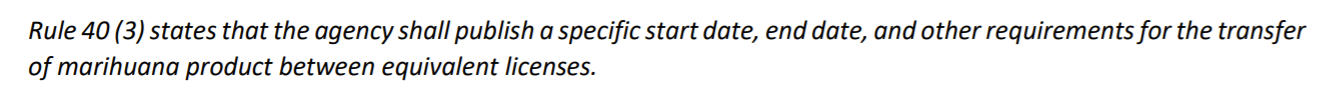
\includegraphics[width=1\textwidth]{images/michigan_transfer_rule_40_3.png}
%\end{center}
\end{frame}


%------------------------------------------------------------------%
% Takeaway
%------------------------------------------------------------------%
\begin{frame}{}
\begin{center}
\begin{minipage}{3.85in}
\begin{block}{Until next time}

\end{block}

\end{minipage}
\end{center}
\end{frame}

%------------------------------------------------------------------%
\end{document}
%------------------------------------------------------------------%
